% =====================================================================
% pipeline_suggestions.tex -- FULL ANNOTATED OVERLAY of main.tex
% ---------------------------------------------------------------------
% main.tex is never modified. This file mirrors it end to end and layers
% corrections on top, so it can be compiled and read side by side.
%
%   % BUILD:     a problem that stops the paper compiling correctly
%   % ACCURACY:  a claim that does not match what the system does
%   % SUGGESTION: a structural or editorial change
%   % WHY-CITE:  why a reference earns its place
%   % KEPT:      your wording, unchanged, noted so you can see what I left alone
%
% Every key resolves against references.bib, suggested_refs.bib, or
% vizij_suggested_refs.bib. No key is invented.
%
% ---------------------------------------------------------------------
% PASS 2 -- against main.tex as of this revision. You adopted most of the
% earlier bullets; these are what is left, most important first.
%
% 1. ACCURACY -- the rewritten Arbitration bullet describes a different design
%    from the one we built. It says the module "receives the outputs of the
%    emotion and viseme generators and combines them into a single set of
%    controller values", with visemes always expressed and emotion "blended in
%    as a secondary layer". Three things are off:
%
%      a) Visemes and emotion never contend. They write DIFFERENT pose channels
%         -- visemes drive the mouth poses, emotion drives its own set -- and
%         the rig composes them when it re-solves. Nothing merges them into one
%         set of values, so there is no precedence to state between them.
%      b) The genuinely contended resource is GAZE, and the bullet no longer
%         mentions it. Turn posture, aversion, joint attention and idle all want
%         the eyes; one slot resolves them by fixed priority, and nods and brow
%         flashes ride on top as impulses without claiming it. That is the part
%         a reader learns something from, and it is what the three citations you
%         dropped (mutlu2009footing, admoni2017social, ribeiro2019nutty) support.
%      c) There IS a real precedence rule between the two EMOTION sources, and
%         it is worth a clause: the robot's own declared affect suppresses
%         mirroring of the partner for a few seconds afterwards. Without that,
%         the face can mirror the partner's expression while saying something
%         that calls for its own -- it contradicts its own words.
%
%    A corrected bullet is below. mutlu2009footing and ribeiro2019nutty are
%    currently cited nowhere in main.tex; the corrected bullet uses them again.
%
% 2. BUILD -- 17 undefined citations remain (12 distinct keys: admoni2017social,
%    edwards2016jali, ekstedt2022vap, elbeleidy2026tutorial,
%    gunes2022reproducibility, mishra2023gaze, schlangen2011iu,
%    skantze2021review, song2023robot, specian2021quori, urakami2023nonverbal,
%    zhou2018visemenet). references.bib is up to 16 entries, so the migration is
%    well along -- these twelve are the remainder, still only in the two
%    suggested bibs. Either finish moving them or point \bibliography at all
%    three files. Careful: several keys are now defined twice, and a repeated
%    entry is a BibTeX *error* that truncates the .bbl and makes EVERY citation
%    read as undefined. paper/merge_bibs.py de-duplicates if you want the
%    shortcut; `make suggestions` uses it.
%
% 3. BUILD -- \ref{fig:demo-screenshot-settings} and
%    \ref{fig:demo-screenshot-pipeline} are still undefined, so the PDF prints
%    "Figures ??, ??". Either add the screenshots or drop the sentence.
%
% 4. The abstract still says recent systems work "from completed dialogue
%    state", and the body still never cites one of them. You chose not to add a
%    related-work subsection, which is a fair call at four pages -- but the
%    claim is currently unsupported anywhere. The minimal fix is one sentence in
%    the Proposal opening with two citations; drafted below, ~40 words. A
%    reviewer who knows FLEX-SDK will otherwise ask.
%
% 5. Typos: "dialoguepartner" -> "dialogue partner"; "wholistic" -> "holistic";
%    "\textit{Sensors}" is missing the period the other bullets have.
%
% 6. The pipeline caption is back to "An illustration of the data pipeline."
%    Your call, but note the boxes in that figure are single words BECAUSE the
%    caption was carrying the detail -- what each stage means and which ones are
%    swappable. As it stands neither the figure nor the caption says it, and the
%    modularity claim is left to the body text alone. Fuller caption below.
% ---------------------------------------------------------------------
% =====================================================================

\documentclass[conference]{IEEEtran}
\IEEEoverridecommandlockouts
\usepackage{cite}
\usepackage{amsmath,amssymb,amsfonts}
\usepackage{algorithmic}
\usepackage{graphicx}
\usepackage{textcomp}
\usepackage{xcolor}
% SUGGESTION: main.tex lacks this; \includegraphics finds the figures without
% it only because they happen to sit in ./figures relative to the build dir.
\graphicspath{{figures/}}
\def\BibTeX{{\rm B\kern-.05em{\sc i\kern-.025em b}\kern-.08em
    T\kern-.1667em\lower.7ex\hbox{E}\kern-.125emX}}

\begin{document}

\title{Vizij $\times$ Retico: A System Architecture for Driving Expressive Robot
Faces from Incremental Dialogue}

\maketitle

% =====================================================================
% ABSTRACT
% KEPT: your abstract, near-verbatim. Two edits only.
% SUGGESTION: the long final-third sentence ran to 34 words and carried two
% ideas; split. "The proposed modular architecture provides a starting point
% for future work to replace and evaluate individual modules" -> the same
% claim, said once.
% =====================================================================
\begin{abstract}
Effective human--robot interaction is both multimodal and incremental, yet
these properties are usually pursued separately: expressive-face systems
render gaze and emotion with no real-time signal to drive them, while
incremental dialogue systems expose no expressive output. We present a system
architecture integrating \textit{retico}~\cite{michael2020retico}, an
incremental framework for real-time spoken dialogue and robot control, with
\textit{Vizij}~\cite{elbeleidy2026vizij}, an open-source framework for
designing, animating, and deploying expressive rendered robot faces. Recent
systems generate robot facial expression from language models, but do so from
completed dialogue state; the architecture described here renders revisable
partial signals mid-utterance. Every stage is substitutable, so the
architecture serves as a platform for evaluating individual modules rather
than as a single demonstration.
\end{abstract}

\begin{IEEEkeywords}
expressive rendered faces, incremental dialogue, social robots
\end{IEEEkeywords}

% =====================================================================
% SUGGESTION: this figure is the one thing that explains what "incremental"
% and "channel" mean to a reader who knows neither system, and both terms are
% load-bearing from the Motivation onward. Place it early -- top of page 1 if
% it will float there, page 2 otherwise.
% =====================================================================
\begin{figure*}[t]
  \centering
  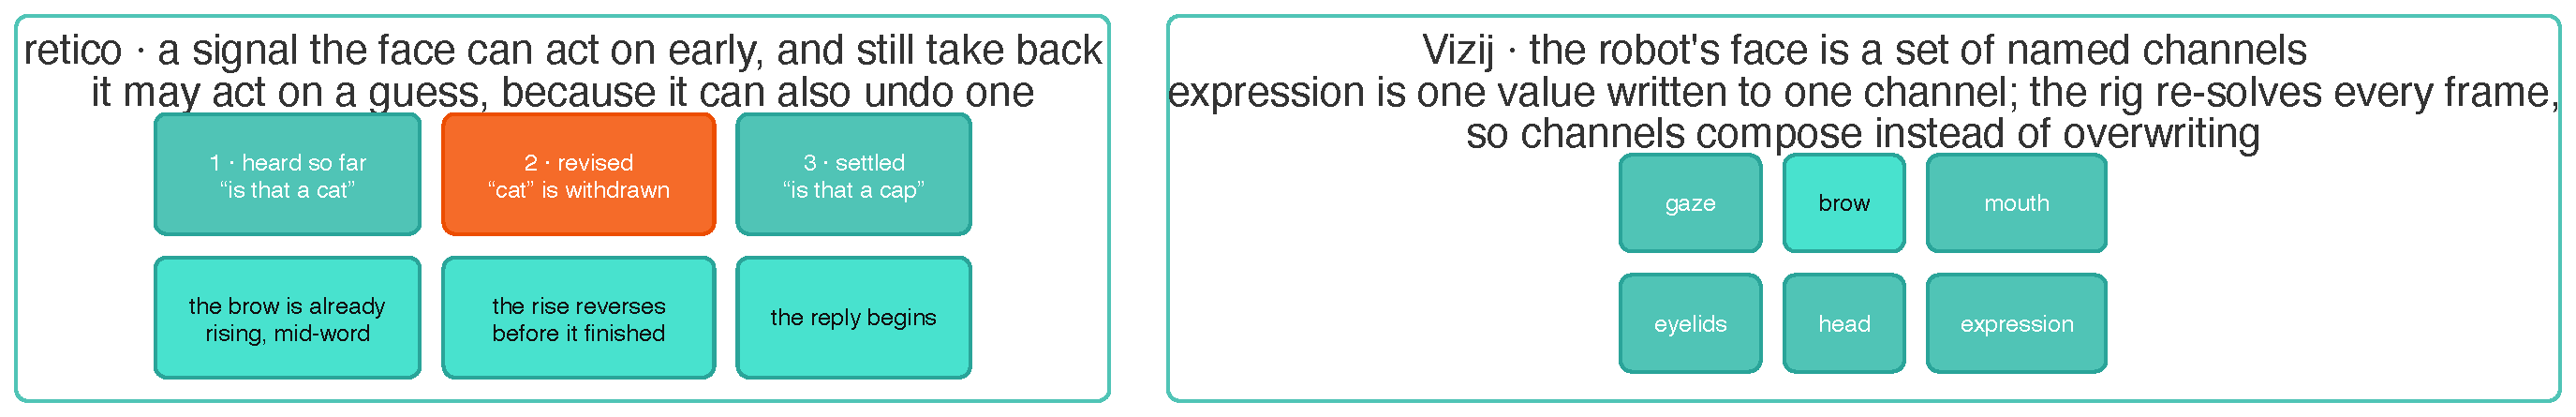
\includegraphics[width=\textwidth]{05_primer.pdf}
  \caption{The two halves. \textbf{Left:} retico contributes signals that are
  revisable --- a partial hypothesis can be added, withdrawn, and replaced ---
  so the face may act on a guess because it can also undo one. \textbf{Right:}
  Vizij contributes a face expressed as named channels rather than as a set of
  pictures; expression is a value written to a channel, and the rig re-solves
  every frame so channels compose instead of overwriting one another.}
  \label{fig:primer}
\end{figure*}

\section{Introduction}

% KEPT verbatim.
Effective Human–Robot Interaction (HRI) must move beyond a unidirectional, listen-and-act paradigm toward genuinely bidirectional dialogue. For safe, trustworthy, and engaging interactions, robots must not only interpret instructions but also ask clarifying questions, signal uncertainty, take turns, explain their behavior, and align with human intent. This work contributes directly to that goal by pairing two open-source systems that together span the full loop such interactions require: (1) retico~\cite{michael2020retico}, an incremental framework for real-time spoken dialogue and robot control, which determines \textit{what} the robot communicates and \textit{when}; and (2) Vizij~\cite{elbeleidy2026vizij,elbeleidy2026tutorial}, a framework for designing, animating, and deploying expressive rendered robot faces, which determines \textit{how} that communication appears—through gaze, visemes, and emotional expression.

\section{Motivation}

% KEPT, with "wholistic" -> "holistic".
Effective Human-Robot Interaction is multimodal and incremental. These two
properties are usually pursued in silos: expressive-face systems render
gaze and emotion agnostic of a signal to drive them, while
incremental dialogue systems evaluate robot behavior agnostic of a holistic multimodal robot expression. Interaction that is responsive in time but expressed on a static face---or expressive in the face but lagging a turn behind---fails in the
same way, because a human partner reads timing and expression together.

\subsection{Robot Expressivity \& Vizij}

% KEPT verbatim.
Dialogue must align with the robot's appearance and expression. What the
robot says is only part of the message, and a face that is static or mistimed
undercuts the spoken content. Nonverbal expressions carry social meaning
alongside speech, and a listener integrates both into a single
interpretation~\cite{urakami2023nonverbal, admoni2017social}. When the two
diverge, for example a face that stays neutral while the robot apologizes, or a face's gaze that remains steady while it yields to the dialogue partner, the nonverbal channel does not simply go unused; it contradicts the words and results in a misaligned dialogue. Alignment is therefore not decoration on top of dialogue but a condition for the dialogue being understood as intended.

% KEPT verbatim.
Expressivity can include a robot face that expresses gaze, visemes, and
emotions effectively and in sync. Each channel does distinct work: gaze
manages turn-taking, coordinates joint attention, and signals cognitive
effort~\cite{mishra2023gaze}; visemes tie articulation to the speech signal so
the face is seen to be speaking~\cite{edwards2016jali}; and emotional expression shapes how users judge trustworthiness and remain engaged~\cite{song2023robot}.

% KEPT verbatim.
\textbf{Vizij:} an open-source ecosystem for designing, animating, and
deploying expressive rendered robot faces~\cite{elbeleidy2026vizij} presents a system that addresses this multichannel communication. It
provides a standardized yet modular rigging and controller system spanning
end-user definable channels such as eye gaze, visemes, and emotional
expression. Vizij enables faces authored to be portable across robot platforms
rather than rebuilt per deployment. What Vizij does not supply is the
moment-to-moment signal that should drive those controllers.

\subsection{Effective Human-Robot Spoken Dialogue}

% KEPT, with "approachare" -> "approach are".
Dialogue is incremental. Speakers plan and articulate in overlapping stages
rather than composing a whole utterance before speaking~\cite{levelt1989speaking},
and listeners develop their interpretations as words arrive~\cite{tanenhaus1995integration}. This is what
makes fast feedback, overlap, and repair possible, and it is why turn-taking
can be predicted continuously from incremental speech rather than
detected after a silence~\cite{skantze2021review, ekstedt2022vap}. Systems
built following this incremental approach are measurably more responsive and are better
received by users~\cite{baumann2011evaluation, kohn2018incremental}.

% KEPT verbatim.
While Large Language Models (LLMs) are increasingly used to generate dialogue, they
process data monotonically. LLMs operate over sentence- or
multi-sentence-level input and cannot revise an interpretation or a partial
output as evidence arrives, which is precisely the capability real-time
interaction demands~\cite{kennington2025prior}. The consequence for a robot is
not merely added latency but a coarser interaction.

% KEPT verbatim.
\textbf{Retico:} addresses this by formalizing an Incremental Unit (IU) framework in which
modules exchange revisable units of information~\cite{schlangen2011iu}. It presents the IU framework as a modular, real-time pipeline in which modules
exchange incremental units, so the system can act on partial input and revise
its decisions as further evidence arrives~\cite{michael2020retico, schlangen2011iu}. Subsequent work extends it toward robots specifically, providing the distributed,
time-aligned, multimodal structure that physical deployment
requires~\cite{kennington2020rrsds, kennington2025retico}.

% =====================================================================
% SUGGESTION (new subsection, ~110 words). This is the largest gap in
% main.tex. The abstract asserts that recent systems "generate robot facial
% expression from language models, but do so from completed dialogue state" --
% and the body never cites one of them, so the paper's central distinction is
% asserted rather than argued. A reviewer who knows FLEX-SDK will also ask why
% the nearest open-source prior art is absent.
%
% WHY-CITE: alvesoliveira2022flexsdk -- face design, expression authoring,
%   Wizard-of-Oz control, scripting. The nearest prior art, and open source.
% WHY-CITE: almoubayed2012furhat -- the reference rendered-face platform.
% WHY-CITE: antony2025xpress, hasumoto2023llmemotion -- language-model-driven
%   expression; exactly the systems the abstract is contrasting against.
%
% CAUTION: do NOT differentiate on "open source". FLEX-SDK is open source and
% that claim will not survive a reviewer who knows it. Differentiate on
% incrementality, which is defensible and is what the system actually does.
% =====================================================================
\subsection{What already exists}

Open-source tooling for rendered faces is not new: FLEX-SDK supports face
design, expression authoring, Wizard-of-Oz control and
scripting~\cite{alvesoliveira2022flexsdk}, and Furhat has served as a
rendered-face platform for over a decade~\cite{almoubayed2012furhat}. Nor is
model-driven expression: recent systems generate facial expression from
language models, per interaction context~\cite{antony2025xpress} or during
live dialogue~\cite{hasumoto2023llmemotion}. What distinguishes the present
work is neither property. Each of those systems consumes \emph{completed}
dialogue state---an utterance, a turn, a context---resolved before an
expression is chosen. None consumes revisable partial signals, and so none can
render a listener response while the partner is still speaking.

\section{Proposal: Vizij $\times$ Retico}

% KEPT verbatim -- this paragraph is the strongest in the draft and needs
% nothing. The three benefits (timing, revisability, reuse) are each accurate.
% SUGGESTION (header item 4): the abstract's contrast, made once, in the body.
% WHY-CITE: alvesoliveira2022flexsdk -- nearest open-source prior art.
% WHY-CITE: antony2025xpress, hasumoto2023llmemotion -- the language-model
%   expression systems the abstract is contrasting against.
% CAUTION: do not differentiate on "open source" -- FLEX-SDK is open source too.
Existing tooling renders robot faces~\cite{alvesoliveira2022flexsdk} and
generates their expression from language
models~\cite{antony2025xpress, hasumoto2023llmemotion}, but each consumes
dialogue state that has already resolved, and so cannot respond while the
partner is still speaking.

In this paper, we present a system architecture integrating Vizij and Retico, so that the robot's expressive face is driven by the same incremental signals that drive its dialogue. This integration results in three key benefits. The first concerns timing: because expressive signals are
available before an utterance concludes, the face can participate during a
partner's turn rather than responding after it, which is the behavior that
distinguishes conversational presence from sequential exchange. The second
concerns revisability: because the provisional status of a signal is preserved
rather than discarded at the boundary between systems, the face may act upon a
hypothesis precisely because it retains the ability to withdraw one. The third
concerns reuse: because the two systems meet through a single specified
interface rather than through mutual accommodation, each component within that
interface can be replaced without disturbing the others, and the architecture
becomes an instrument for comparison rather than a single demonstration.

The proposed interaction pipeline includes the following components:
\begin{itemize}
  % KEPT verbatim.
  \item \textit{Sensors.} The robot senses its dialogue partner's speech through the microphone and their emotional expression through the camera.

  % ACCURACY: this is the important one. Your text reads "estimates when the
  % robot should speak based on what the dialogue partner has said so far",
  % which describes a module that consumes recognised words. Voice Activity
  % Projection consumes the AUDIO SIGNAL and runs in parallel with recognition.
  % That distinction is the whole mechanism: if turn-taking waited on words it
  % could not produce a signal before a transcript exists, and the timing
  % benefit claimed in the paragraph above would not follow.
  \item \textit{Turn-taking.} The turn-taking module continuously estimates
        when the robot should speak from the audio signal
        directly~\cite{skantze2021review, ekstedt2022vap}. It runs in parallel
        with recognition rather than downstream of it, so a turn estimate is
        available before any transcript exists.

  % KEPT, with one clarification: "added, withdrawn, or confirmed" is exactly
  % right and is genuinely what the recogniser emits -- worth stating plainly
  % that this is per word, since that is what makes it incremental.
  \item \textit{Incremental speech recognition.} The speech recognition module emits
        partial hypotheses as it determines what the dialogue partner is saying,
        labelling each as added, withdrawn, or
        confirmed, so that downstream modules receive not only the current
        interpretation but its epistemic standing~\cite{schlangen2011iu,
        michael2020retico}.

  % SUGGESTION: expand very slightly. As written this is one clause and reads
  % as a placeholder next to the others.
  \item \textit{Incremental dialogue production.} The reply is generated as a
        stream and split into clauses, each of which is synthesised and sent to
        the face as it is produced rather than after the reply completes.

  % ACCURACY / CLARITY: the original conflates the two emotion paths and the
  % phrase "for each incremental unit of speech" is ambiguous about whose
  % speech. There are two distinct sources with different provenance, and the
  % honest framing separates them -- the first is the robot's INTENDED affect,
  % declared by the model generating the words, not perceived from anything.
  \item \textit{Emotion generation.} Two sources drive expression. The robot's
        own affect is declared by the dialogue model at the start of each
        reply clause, so the face is set as that clause begins to be spoken
        rather than after the reply ends. Separately, the dialogue partner's expression
        is estimated from the camera and mirrored faintly.

  % ACCURACY: "calculated based on the confirmed speech unit to produce" reads
  % as though visemes derive from the RECOGNISED speech. They derive from the
  % robot's own outgoing speech -- the synthesiser's phoneme timings for the
  % clause it is about to speak. Worth stating unambiguously, because a reader
  % who assumes the former will wonder why the robot's mouth follows the
  % partner's words.
  \item \textit{Viseme generation.} Mouth shapes follow the robot's own
        outgoing speech. Where the synthesiser reports phoneme timings, they
        drive the mouth poses directly~\cite{edwards2016jali,
        zhou2018visemenet}; where it does not, mouth opening follows the
        amplitude of the playing audio as a fallback.

  % ACCURACY: see header item 1. Restores gaze as the contended resource and
  % adds the emotion-source precedence rule, which is real and currently unsaid.
  \item \textit{Arbitration and rendering.} Channels that more than one signal
        wants are assigned to a single occupant by fixed precedence. Gaze is the
        contested case---turn posture, aversion, and joint attention all want
        the eyes---while brief impulses such as nods and brow flashes are
        composed over the sustained posture rather than displacing
        it~\cite{mutlu2009footing, admoni2017social, ribeiro2019nutty}. The two
        emotion sources are ordered rather than mixed: the robot's own declared
        affect suppresses mirroring of the partner for several seconds, so the
        face does not reflect the partner's expression while saying something
        that calls for its own. Visemes and emotional expression need no
        arbitration, as they drive separate channels that the rig composes.
\end{itemize}

% SUGGESTION: the caption in main.tex is "An illustration of the data
% pipeline." A figure this central should be readable without the body text;
% the caption is also where the substitutable stages can be enumerated without
% costing type size inside the diagram.
\begin{figure*}[t]
  \centering
  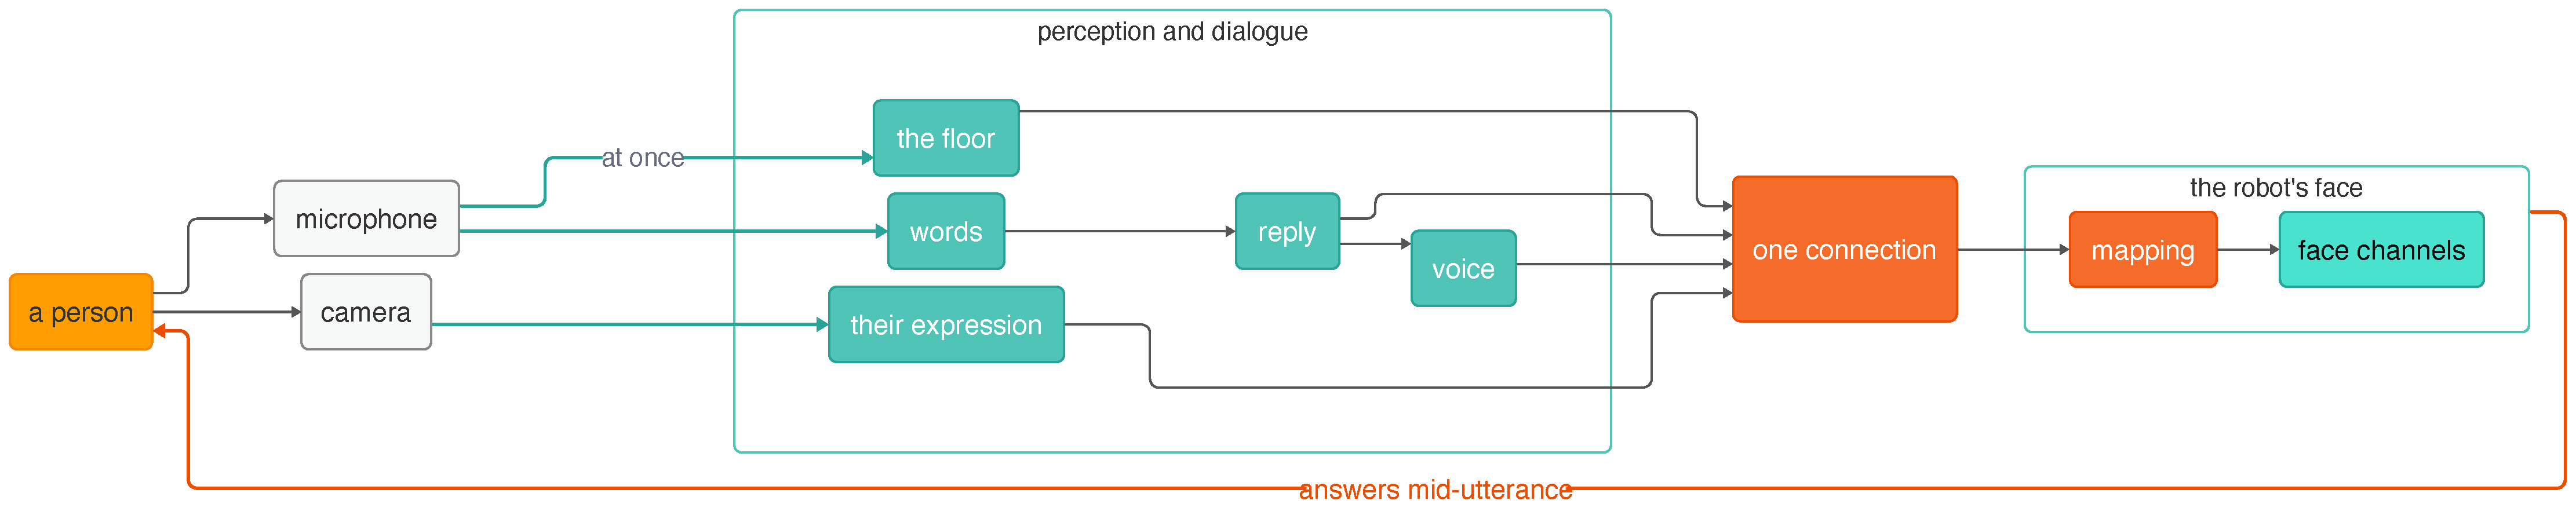
\includegraphics[width=\textwidth]{06_pipeline_simple.pdf}
  \caption{The pipeline. Microphone audio reaches \emph{the floor} (is a turn
  ending? is now a moment to nod?) and \emph{words} at the same instant rather
  than in sequence, which is why a listener response can be rendered before a
  transcript exists. Every teal stage is a provider chosen at run time ---
  words from an on-board or a cloud recogniser, expression from either of two
  vision models, reply from any OpenAI-compatible chat model whether local or
  hosted, voice from any of three synthesisers --- and availability is
  computed from the environment, so an unconfigured provider appears disabled
  rather than failing when selected. \emph{Mapping} is the editable table that
  decides which signal moves which channel, and how fast.}
  \label{fig:pipeline}
\end{figure*}

% KEPT verbatim.
We implemented this pipeline in a modular approach that allows the developer / designer / researcher to swap out different modules and evaluate their impact. The
significance of this is methodological rather than merely practical.
Substituting one component while holding the remainder fixed enables thorough scientific evaluation of the modified component and reproducible comparison with the original. Our proposed architecture is therefore not only a demonstration of a single system but also a platform for future work to evaluate and compare individual modules or module combinations.

% SUGGESTION: one concrete measurement earns this paragraph its keep. Without
% it "modularity enables comparison" is a claim about a hypothetical.
% MEASURED: 2.5-flash-lite (regional endpoint) 0.40 s to first token vs
%   3.5-flash-lite (global-only endpoint) 1.04 s, everything else held fixed.
%   Name the models if you want it checkable; left generic so the paper is not
%   read as being about one vendor.
A single substitution illustrates the point. Exchanging only the dialogue
model, with every other stage fixed, moved median time-to-first-token from
$0.40$\,s to $1.04$\,s---and the newer model was the slower of the two,
because it is served only from a geographically general endpoint whose routing
cost exceeded the model's advantage. Where a model is served can matter more
than which model it is, and that is a comparison this architecture makes cheap
to run.

% BUILD: \ref{fig:demo-screenshot-settings} and \ref{fig:demo-screenshot-pipeline}
%   are undefined -- those figures do not exist yet. Either add them or drop
%   the sentence; as it stands the PDF prints "Figures ??, ??".
% TYPOS: "publically" -> "publicly"; "throught" (earlier bullet) -> "through".
% SUGGESTION: keep the web-demo sentence short and unapologetic. The browser
% is how this instance is deployed, not what the architecture is; the rest of
% the paper speaks in sensors, and this is the one place that has to reconcile
% the two.
We developed this pipeline as a web-based demonstration, using the browser's
microphone and camera in place of the robot's sensors and rendering the
publicly available Quori~\cite{specian2021quori} face.
%A screenshot of the demo is shown in Figures~\ref{fig:demo-screenshot-settings},~\ref{fig:demo-screenshot-pipeline}.
%The demo is available at \url{https://vizij.ai/retico-demo}.

% =====================================================================
% SUGGESTION (new section, ~200 words). main.tex goes Proposal -> Conclusion
% with no limitations anywhere. For a systems paper with no user study, stating
% the bounds yourself is what keeps a reviewer from stating them for you, and
% it costs less than a quarter page.
% =====================================================================
\section{Discussion}

% WHY-CITE: broadbent2013screenface, longface2026 -- display geometry and
%   physicality change how a face is read.
% WHY-CITE: hartholt2019vhtoolkit -- precedent for one behaviour pipeline
%   driving several embodiments; supports the ambition without overclaiming.
Portability here is a claim about the value stream, not about perception.
Display geometry, proportion, and physicality are known to change how a face
is read~\cite{broadbent2013screenface, longface2026}, so an identical channel
stream rendered on a physical platform is not an identical face. Driving
several embodiments from one behaviour pipeline is established
practice~\cite{hartholt2019vhtoolkit}; establishing that they are
\emph{perceived} alike is a separate empirical question.

% SUGGESTION: three limitations, stated plainly. Each is real.
Three limitations bound what is claimed. The robot's affect is declared by the
model generating its words rather than derived from a model of its own state,
and the partner's expression is estimated categorically and coarsely.
Turn-taking and listener-cue quality is inherited entirely from the upstream
predictors---this architecture renders those signals, it does not improve
them. And there is no user study: every claim here is a claim about the
system, not about its effect on people.

% SUGGESTION (deferred): the evaluation figure. Uncomment once a session has
% been recorded. The caption is written first on purpose -- stating in advance
% what the figure must show keeps the measurement honest about what it needs
% to produce. Do not sketch hoped-for data in the meantime.
%
% \begin{figure}[t]
%   \centering
%   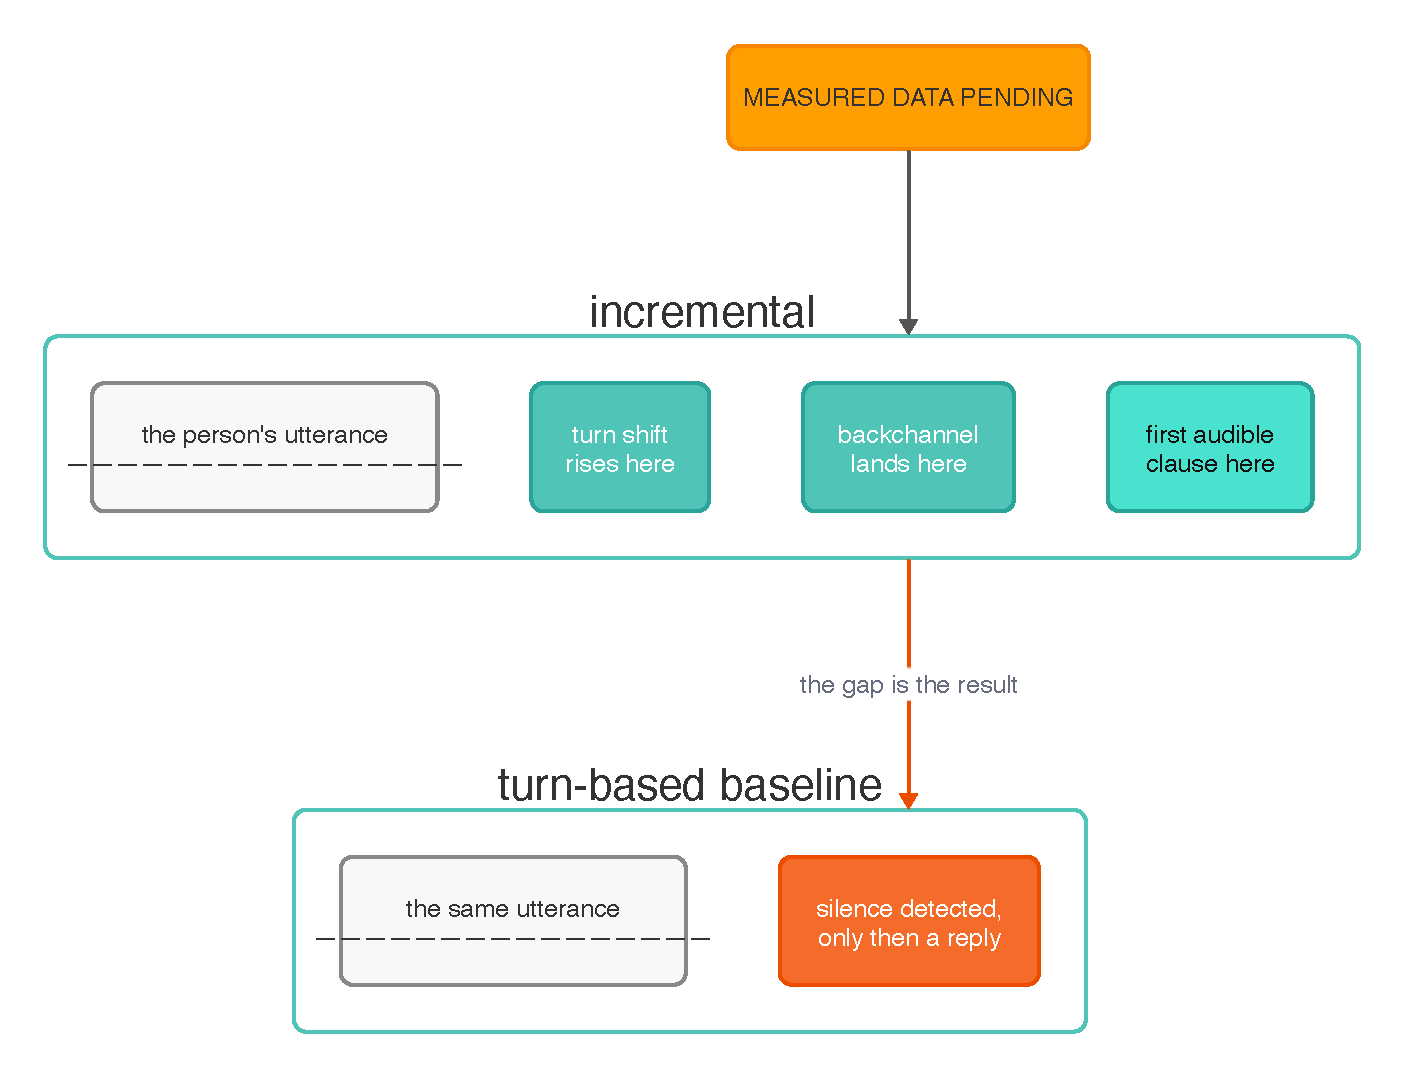
\includegraphics[width=\columnwidth]{07_timeline.pdf}
%   \caption{Social signals land during the partner's utterance. Turn-shift
%   probability, the listener cue, and the first audible clause are plotted
%   against the utterance; a turn-based baseline can respond only after the
%   silence at the end.}
%   \label{fig:timeline}
% \end{figure}

\section{Conclusion}

% KEPT verbatim.
In this paper, we described an architecture that couples incremental spoken dialogue to
an expressive robot face. The dialogue system, retico, determines what is communicated
and when, and the face system, vizij, determines how that communication appears. The architecture enables robot expression to begin
before an utterance is complete and be withdrawn should the collected evidence change.
Both systems we integrate are open source and each module within the pipeline is substitutable, which makes the proposed architecture a testbed rather than a simple demonstration---a form of
contribution the field has argued it requires more
of~\cite{gunes2022reproducibility}. We hope this work will enable future research to evaluate the impact of individual modules or module combinations on the quality of human-robot interaction.

% KEPT verbatim -- added to main.tex after this overlay was started. Good
% practice, and increasingly expected; no changes suggested.
\section{AI Use Disclosure}
The authors used generative AI tools to assist in the writing of the paper and identifying relevant references. The authors provided an original outline to limit the AI's influence on the content then verified and re-wrote the resulting output.

% =====================================================================
% BUILD -- THE MOST IMPORTANT LINE IN THIS FILE.
% main.tex has \bibliography{references}, and references.bib contains only
% michael2020retico and elbeleidy2026vizij. The other nineteen cited keys are in
% the two suggested bibs, so they resolve to nothing: 31 undefined-citation
% warnings, and a reference list with two entries in it. Listing all three files
% fixes every one of them. Merging the suggested bibs into references.bib and
% keeping {references} works equally well -- just do one or the other.
% =====================================================================
\bibliographystyle{IEEEtran}
\bibliography{merged_refs}

\end{document}
